\documentclass{article}
\usepackage{amsmath} % equation, align, matrix, *, &, \\, \left, \right
\usepackage{graphicx} % figure
\usepackage{subcaption} % subfigure
\usepackage{comment} % To comment
\usepackage{hyperref} % To hyperlink and ref
\usepackage{enumitem} % To list
%\usepackage[ngerman]{babel}
\usepackage[utf8]{inputenc}
\usepackage{wrapfig}
\usepackage{ulem}
\usepackage[backend=bibtex,style=numeric]{biblatex}
\usepackage{subfiles} %multifile latex projects
\usepackage{multirow}
\usepackage{booktabs}
\usepackage{csquotes}
\usepackage[section]{placeins}
\usepackage{color,soul}

%\usepackage{fontspec}
\graphicspath{{images/}{../images/}}

\bibliography{lib} 

\title{IoT System Project - Irrigation Sprinkler}
\author{Tim Reiprich, Tegshigzugder Otgonbayar}

\begin{document}

\pagestyle{plain} \pagenumbering{gobble} %hide page numbers

\maketitle
% \section{}
% \subsection{}
% \subsubsection{}

% \paragraph{}
% \subparagraph{}

\newpage

\pagenumbering{arabic} %show page numbers in arabic
\tableofcontents % from the section headings
\newpage

% \listoffigures \listoftables
% \newpage
\section{Introduction}
In the summer season, one of the crucial tasks for people in the agricultural field is to provide sufficient water to their crops but also not to overwater. Therefore we have chosen to develop an IoT System Project for managing and regulating irrigation sprinklers automatically and smartly. The use case can be also extended to people for residential and industrial usage.

\section{General description}
In our project, we have three main sensors: light sensor, temperature sensor, and distance sensor. Each sensor has an independent function. Furthermore, there is a possibility to combine these sensors for more complex usage.
In the following the independent functions of the sensors are described:
\begin{itemize}
\item Light sensor: to sense if it is day or night so that we can decide when to activate the sprinklers
\item Temperature sensor: to sense how warm the temperature is so that the sprinklers are distributing water for a longer or shorter time
\item Distance sensor: to sense if an object such as a door is open or closed so that the sprinklers turn off e.g. if a person enters the field
\end{itemize}

For the development of this project, we have mainly used the applications and tools introduced in the course. Due to do the current pandemic we have opted to build the circuit in the online simulator TinkerCAD instead of a physical circuit. This also enabled us easily to work together. The source code is to be found in our GitHub repository \url{https://github.com/ajpqa/iot2}. The hardware scheme is to be found under \url{https://www.tinkercad.com/things/9b2RV6Rs0I2-projectfinal}.
\section{Hardware Scheme}
In this part, we will describe the scheme of our project, which is to be seen in Figure \ref{fig:scheme}. It consists of an Arduino Uno R3 which functions as a micro-controller and collects data of the environment to control the sprinklers. The sensors to collect data are TMP36 (a temperature sensor), HC-SR04 (a distance sensor), and Photoresistor (a light sensor). The temperature is measured because the plants need more water if it's warmer and less if the temperature isn't that high. Furthermore, the light sensor is used to determine a good day time to water the plants. Preferably it should always happen in the evening or night as there is a higher chance people work there during the day and plants can get \enquote{burned} if there is strong sunlight that gets amplified by water drops on the plants. And lastly, we use a distance sensor to determine if the door to the greenhouse is open or closed. If it is open there are workers inside which means that the sprinklers have to be turned off. Only after the door is closed the sprinkler can be turned on again.\par
The last component of the hardware scheme is the ESP8266 Wifi module which is used to send the measured data to a user interface and Google Cloud by using the MQTT protocol. Unfortunately, the Tinkercad circuit simulator doesn't support the Arduino library \texttt{PubSubClient.h} which leads to us not being able to test our configuration completely. For this, the limitations of the simulator are too narrow. In theory, the developed code will work in a real environment and as a solution, we have provided a python script to simulate the sending of the data to the MQTT broker so that the circuit, the user interface, and the evaluation of collected data work well with Google Cloud however the transmission of the data has to be additionally simulated by executing the python script.
\begin{figure}
\centering
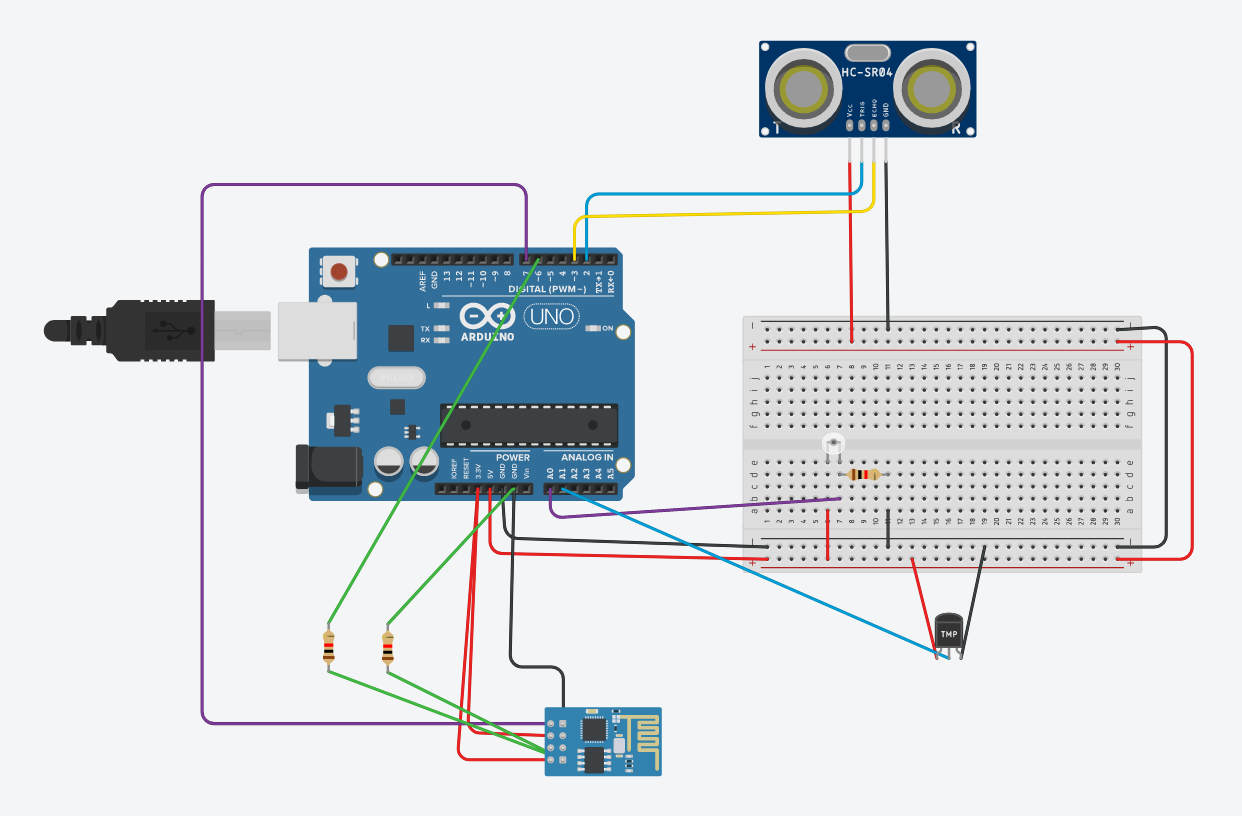
\includegraphics[scale=0.3]{scheme_cropped.png}
\caption{Circuit that was built during the project}
\label{fig:scheme}
\end{figure}
\section{Implementation}
The implementation of the project was written in the programming languages C++ and Python. The project consists of the following main parts:
\begin{itemize}
\item project.ino - program for the micro-controller
\item mqtt.py - the mqtt simulation and virtual environment
\item main.py - the user interface for the local view and control of sensors and sprinklers
\end{itemize}
\subsection{project.ino}
The project.ino file contains the code controlling the Arduino. Its main purpose is to collect the sensor data and convert it to humanly standardized measurements. Thus the data is sent via MQTT to a broker. \par
This file consists of multiple functions. The following two additional helper functions were written; \texttt{sendData} handles sending commands to the ESP8266 Wifi module and \texttt{readUltraSonicDistance} handles measuring the distance as it requires relatively more than the other sensors. The two basic functions are \texttt{setup()} and \texttt{loop()}. \texttt{setup()} initializes all variables and sets up the connection to the Wifi while \texttt{loop()} periodically gets the sensors' measurements, prints them to the serial monitor and finally converts the data into a JSON and publishes it via MQTT. Due to restrictions of the Tinkercad simulator, the last part can't be used in the simulator as the MQTT library is not available there. Additionally, the Wifi module itself is no longer supported because of security reasons (see figure \ref{fig:security}). There is also a library which should make it easier to establish a Wifi connection using the ESP8266 but it also not supported in the simulator. So finally, the code regarding MQTT and the Wifi library are in the file as comments. It should work in a real environment but it can't be tested in the simulator. Furthermore, we created a python file \texttt{mqtt.py} as a workaround which simulates the publishing of the data, which is explained in the next chapter.\par
\begin{figure}
    \centering
    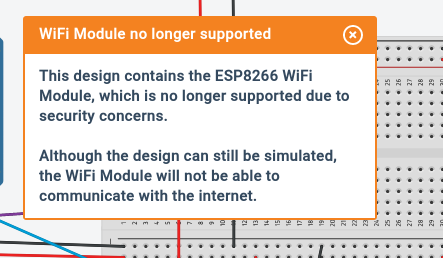
\includegraphics[scale=0.4]{security.png}
    \caption{Notice regarding the ESP8266 in Tinkercad}
    \label{fig:security}
\end{figure}
\subsection{mqtt.py}
This is an additional file that would not be needed if we would have used a real circuit but due to the special circumstances, we use it to simulate publishing the measured data via MQTT. It simply contains three functions each simulating a sensor and publishes the \enquote{measured} data to the Google Cloud Platform and the HiveMQ MQTT broker where the user interface gets its data from.
\subsection{main.py}
The User Interface is to be found here. It was mainly created with the widgets of tkinter and tkkinter. It consists of the following three pages; control, value, and summarize.
\paragraph{Control page}
Here are the main control and view of the system. In the "Sensors control" box we can start or stop the receiving of the values of the sensors. In this case, depending on a boolean value the received values of the subscription are either inserted or not. In the "Current" values box the most recent received values are shown. The main feature of the distance sensor is to stop the sprinklers in the case that a person or object is moving to the field. In "Automatic Stop" we can set a distance threshold when the trigger object is too close. For example, if the object is a door and the door is opened, the sprinkler stops for a period of time until the door is closed again. Here the status is either "Under Threshold" or "Over Threshold". By clicking on the "Confirm" button we can set a new distance threshold.
\begin{figure}
\centering
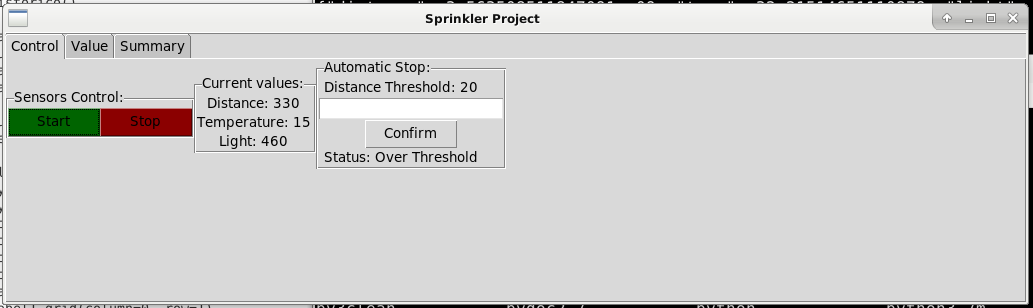
\includegraphics[scale=0.3]{control_view.png}
\caption{Control Page}
\label{fig:control}
\end{figure}
\paragraph{Value page}
While in the "Control" page we can only see the most recent values, in the "Value" page all of the values are registered. This can be useful for further analyzing and evaluating based on the specific needs of the user.
\begin{figure}
\centering
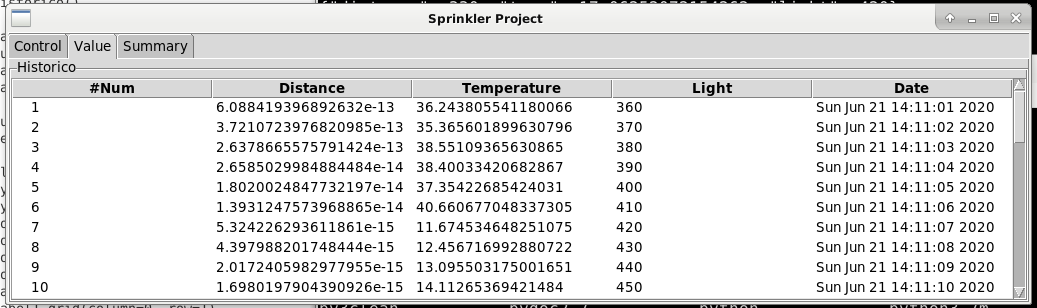
\includegraphics[scale=0.3]{value_view.png}
\caption{Value page}
\label{fig:value}
\end{figure}
\paragraph{Summarize page}
The summarize page functions to evaluate the values. With the "Summarize" button the average "temperature" and "light" values are calculated.
\begin{figure}
\centering
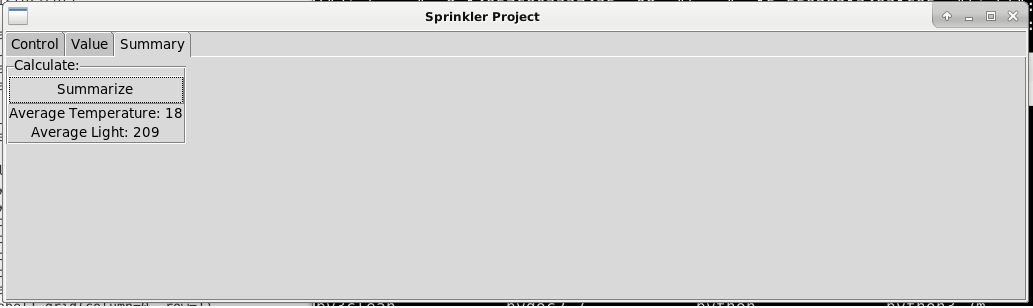
\includegraphics[scale=0.3]{summarize_view.png}
\caption{Summarize page}
\label{fig:summarize}
\end{figure}

\section{Mango}
Additionally to the Tkinter user interface we also created a simple user interface usign Mango which runs in a virtual machine using Compute Engine of the Google Cloud Platform

\section{Google Cloud Platform}
To be able to store the measured data for later analysis we decided to use the Google Cloud Platform as it provides enough storage as well as multiple tools to analyse the stored data.\par
We used a similar approach to the class. We created a new registry and device to receive the data via MQTT using the Pub/Sub tool provided by the Google Cloud Platform. As seen in figure \ref{pic:messages} the data is received successfully.\par
\begin{figure}
\centering
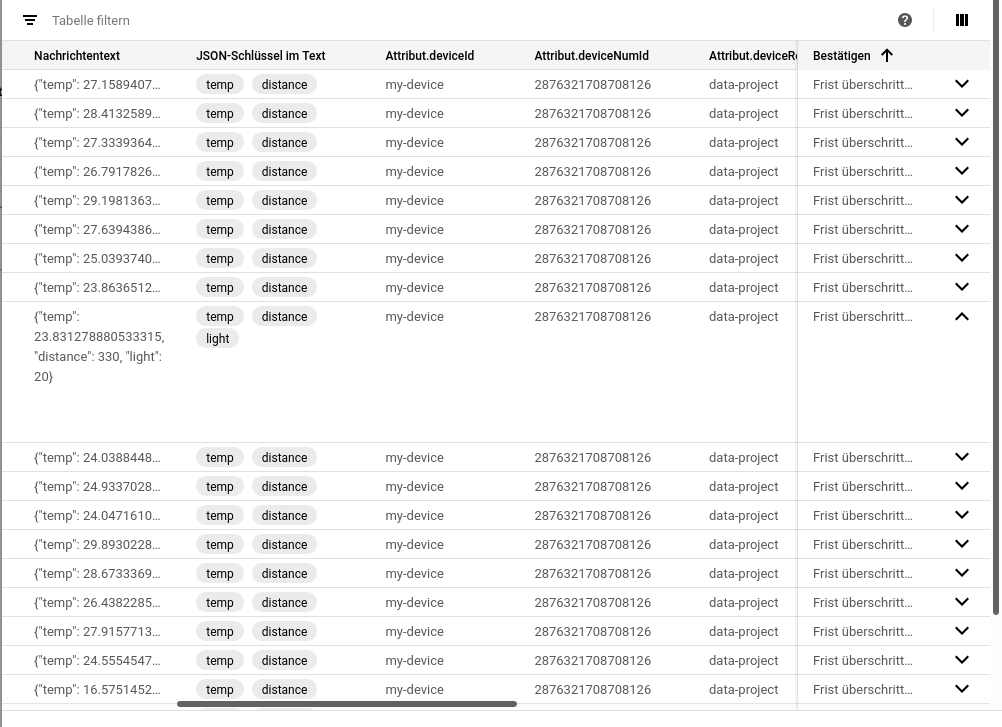
\includegraphics[scale=0.4]{messages.png}
\caption{Received messages via the Pub/Sub tool}
\label{pic:messages}
\end{figure}
To permanently store the received data we used a Cloud Function to store the data in a SQL table which we created using BigQuery, as to be seen in Figure \ref{fig:table}).
\begin{figure}
\centering
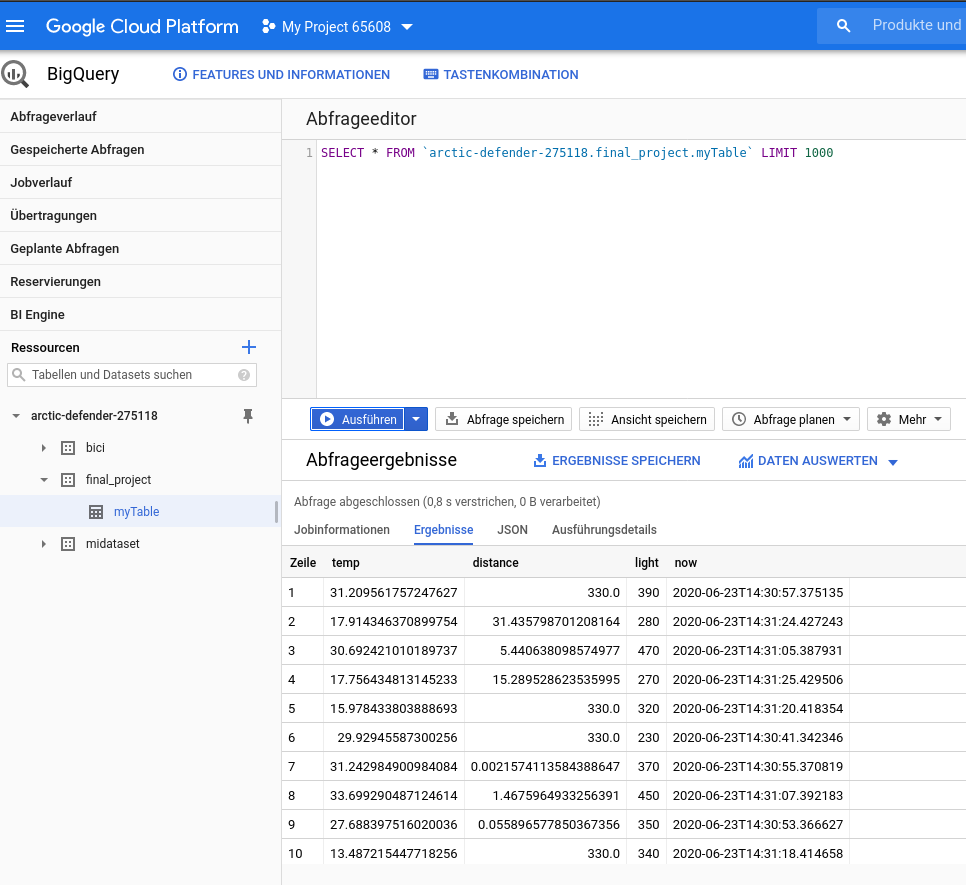
\includegraphics[scale=0.4]{table.png}
\caption{Stored measurements in a BigQuery table}
\label{fig:table}
\end{figure}
From there it can be easily extracted to either look at certain data points or analyze it using further tools.
\subsection{Mango}
Additionally we also created a simple user interface using Mango which runs in a virtual machine using Compute Engine. This interface can be accessed through the internet without having any programs running locally. So if for whatever reason it is not possible to run the Tkinter interface, we wanted to privide another solution as backup. As it is not intended to be the main interface, it only shows the current measured values as a general overview. It can be seen in figure \ref{fig:mango}
\begin{figure}
    \centering
    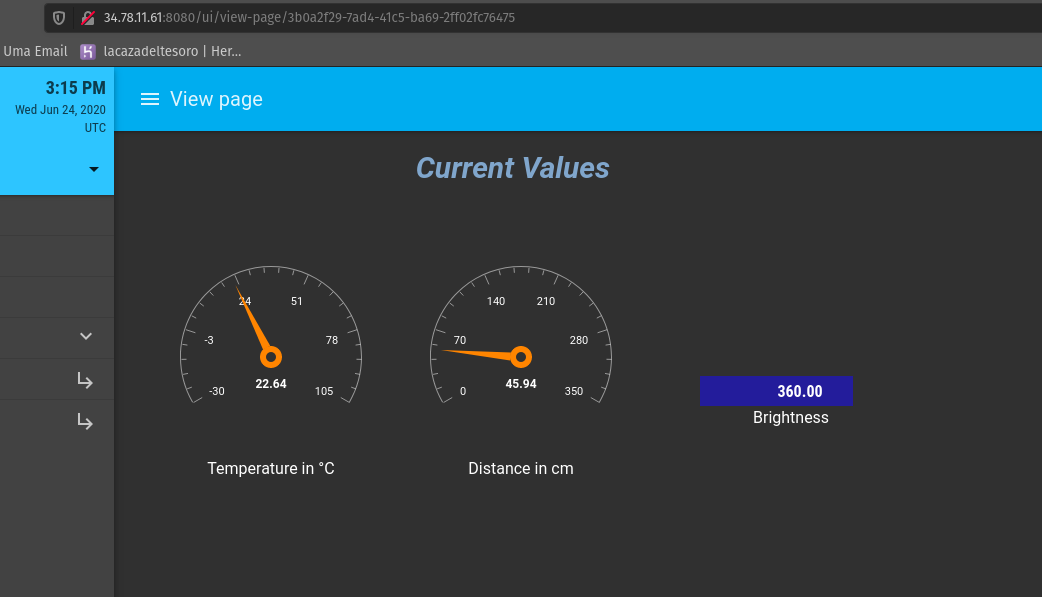
\includegraphics[scale=0.35]{mango.png}
    \caption{User Interface created using Mango}
    \label{fig:mango}
\end{figure}
\section{Summary}
In this document, we have presented our developed IoT System Project for irrigation sprinklers. We have built the circuit in TinkerCAD, which collects data from the sensors. Thus the data from the sensors are used to provide data for our user interface, for a local view of the data and control of the sprinklers, and Google Cloud Console, for further complex data storage and evaluation. There were some difficulties due to the current pandemic that we could not work with actual physical hardware. However, we are confident that our system will run on real environment hardware with a few fixes. \newline
It was enjoyable to work on the project as a team and to implement our personal idea into a practical solution was great. This project gave us a great opportunity to work and further practice the tools and technologies we have reviewed in the course. There are more possibilities to enhance the system such as; more components like LED and Battery to provide further feedback and portability to the device. On the software side, the user interface can be improved by being able to set exact attributes on how to run the system and sprinklers. Also by communicating with actual people who work in this agricultural field, more personalized and needed data can be illustrated. Nonetheless, we believe that the core and main functions of the system are considered and presented.

\end{document}
